\documentclass[11pt,a4paper,oneside]{book}
\usepackage{umcu}
\title{SPARQLing structural variation}
\author{Roel Janssen}

\begin{document}

\begin{titlepage}
  \topskip0pt
  \vspace*{\fill}
  \begin{center}
    \rule{\textwidth}{1.0pt}~\\~\\
    \Huge SPARQLing structural variation
    \rule{\textwidth}{1.0pt}
    \Large Roel Janssen~\\~\\
    \large September 2017
    % Put it a little bit above the center of the page.
    ~\\~\\~\\~\\~\\~\\~\\~\\~\\~\\~\\~\\~\\~\\
  \end{center}
  \topskip0pt
  \vspace*{\fill}

  \thispagestyle{empty}
\end{titlepage}

\setcounter{page}{1}
\pagenumbering{roman}
\hypersetup{linkcolor=black}
\tableofcontents
\newpage{}
\hypersetup{linkcolor=LinkGray}
\setcounter{page}{1}
\pagenumbering{arabic}

\chapter{Getting started}

  SPARQLing genomics is a combination of tools and practices to create a
  knowledge graph to make \emph{discovering}, \emph{connecting}, and
  \emph{collaborating} easy.

\section{Prerequisites}
\label{sec:prerequisites}

  The programs provided by this project are designed to build a knowledge graph.
  However, a knowledge graph store (better known as an RDF store) is not included
  because various great RDF stores already exist, including
  \href{https://virtuoso.openlinksw.com/}{Virtuoso},
  \href{https://github.com/4store/4store}{4store} and
  \href{https://www.blazegraph.com/}{BlazeGraph}.  We recommend using one of
  the mentioned RDF stores with the programs from this project.

  Before we can use the programs provided by this project, we need to build
  them.  The build system needs
  \href{https://www.gnu.org/software/autoconf}{GNU Autoconf},
  \href{https://www.gnu.org/software/automake}{GNU Automake},
  \href{https://www.gnu.org/software/make}{GNU Make} and
  \href{https://www.freedesktop.org/wiki/Software/pkg-config/}{pkg-config}.
  Additionally, for building the documentation, a working \LaTeX{} distribution is
  required including the \texttt{pdflatex} program.  Because \LaTeX{} distributions
  are rather large, this is dependency is optional, at the cost of not being able
  to (re)generate the documentation.

  Each component in the repository has its own dependencies.  Table
  \ref{table:dependencies} provides an overview for each tool.  A \B{}
  indicates that the program (row) depends on the program or library (column).
  Care was taken to pick dependencies that are widely available on GNU/Linux
  systems.

  \hypersetup{urlcolor=black}
  \begin{table}[H]
    \begin{tabularx}{\textwidth}{X *{9}{!{\color{white}\VRule[1pt]}l}}
      \headrow \cellcolor{White}
      & \rotatebox[origin=l]{90}{\href{https://gcc.gnu.org/}{C compiler}\space\space\space}
      & \rotatebox[origin=l]{90}{\href{http://www.librdf.org/}{raptor2}}
      & \rotatebox[origin=l]{90}{\href{http://www.xmlsoft.org/}{libxml2}}
      & \rotatebox[origin=l]{90}{\href{http://www.htslib.org/}{HTSLib}}
      & \rotatebox[origin=l]{90}{\href{https://zlib.net/}{zlib}}
      & \rotatebox[origin=l]{90}{\href{https://www.gnu.org/software/guile}{GNU Guile}}
      & \rotatebox[origin=l]{90}{\href{https://www.gnutls.org/}{GnuTLS}}
      & \rotatebox[origin=l]{90}{\href{https://tug.org/texlive/}{\LaTeX{}}}\\
      \evenrow
      \texttt{vcf2rdf}         & \B & \B &    & \B &    &    & \B &\\
      \oddrow
      \texttt{bam2rdf}         & \B & \B &    & \B &    &    & \B &\\
      \evenrow
      \texttt{table2rdf}       & \B & \B &    &    & \B &    & \B &\\
      \oddrow
      \texttt{json2rdf}        & \B & \B &    &    & \B &    & \B &\\
      \evenrow
      \texttt{xml2rdf}         & \B & \B & \B &    & \B &    & \B &\\
      \oddrow
      \texttt{folder2rdf}      &    &    &    &    &    & \B &    &\\
      \evenrow
      \texttt{sg-web}          &    &    &    &    &    & \B & \B &\\
      \oddrow
      \texttt{sg-web-test}     &    &    &    &    &    & \B & \B &\\
      \evenrow
      \texttt{sg-auth-manager} &    &    &    &    &    & \B & \B &\\
      \oddrow
      Documentation            &    &    &    &    &    &    &    & \B \\
    \end{tabularx}
    \caption{\small External tools required to build and run the programs of
      this project.}
    \label{table:dependencies}
  \end{table}
  \hypersetup{urlcolor=LinkGray}

  The manual provides example commands to import RDF using
  \href{https://curl.haxx.se/}{cURL}.

\section{Installing the prerequisites}

\subsection{Debian}

  Debian includes all tools, so use this command to install the
  build dependencies:

\begin{siderules}
\begin{verbatim}
apt-get install autoconf automake gcc make pkg-config zlib1g-dev  \
                guile-2.2 guile-2.2-dev libraptor2-dev libhts-dev \
                texlive curl libxml2-dev gnutls-dev
\end{verbatim}
\end{siderules}

  This command has been tested on Debian 10.  If you're using a different
  version of Debian, some package names may differ.

\subsection{CentOS}

  CentOS 7 and 8 do not include \texttt{htslib}.  Follow the instructions on
  the \href{https://www.htslib.org/}{\texttt{htslib} website}%
  \footnote{https://www.htslib.org/} to build \texttt{htslib} from source.

  All other dependencies can be installed using the following command:

\begin{siderules}
\begin{verbatim}
yum install autoconf automake gcc make pkgconfig guile guile-devel \
            raptor2-devel texlive curl libxml2-devel gnutls-devel
\end{verbatim}
\end{siderules}

\subsection{GNU Guix}

  For GNU Guix, use the \texttt{environment.scm} file to set up the development
  environment:

\begin{siderules}
\begin{verbatim}
guix environment -l environment.scm
\end{verbatim}
\end{siderules}

\subsection{MacOS}

  The necessary dependencies to build \texttt{sparqling-genomics} can be
  installed using \href{https://brew.sh/}{homebrew}:

\begin{siderules}
\begin{verbatim}
brew install autoconf automake gcc make pkg-config guile \
             htslib curl raptor libxml2 zlib gnutls
\end{verbatim}
\end{siderules}

  Due to a missing \LaTeX{} distribution on MacOS, the documentation
  cannot be build.

\section{Obtaining the source code}
\label{sec:obtaining-tarball}

  \begin{sloppypar}
  The source code can be downloaded at the
  \href{https://github.com/UMCUGenetics/sparqling-genomics/releases}%
  {Releases}%
  \footnote{\url{https://github.com/UMCUGenetics/sparqling-genomics/releases}}
  page.  Make sure to download the {\fontfamily{\ttdefault}\selectfont
    sparqling-genomics-\sgversion{}.tar.gz} file.
  \end{sloppypar}

  Or, directly download the tarball using the command-line:
\begin{siderules}
\begin{lstlisting}[language=bash]
curl -LO https://github.com/UMCUGenetics/sparqling-genomics/releases/\
download/(@*\sgversion{}*@)/sparqling-genomics-(@*\sgversion{}*@).tar.gz
\end{lstlisting}
\end{siderules}

  After obtaining the tarball, it can be unpacked using the \texttt{tar}
  command:

\begin{siderules}
\begin{lstlisting}
tar zxvf sparqling-genomics-(@*\sgversion{}*@).tar.gz
\end{lstlisting}
\end{siderules}

\section{Installation instructions}

  After installing the required tools (see section \refer{sec:prerequisites}),
  and obtaining the source code (see section \refer{sec:obtaining-tarball}),
  building involves running the following commands:

\begin{siderules}
\begin{lstlisting}
cd sparqling-genomics-(@*\sgversion{}*@)
autoreconf -vif # Only needed if the "./configure" step does not work.
./configure
make
make install
\end{lstlisting}
\end{siderules}

  To run the \texttt{make install} command, super user privileges may be
  required.  This step can be ignored, but will keep the tools in the project's
  directory.  So in that case, invoking \texttt{vcf2rdf} must be done using
  \texttt{tools/vcf2rdf/vcf2rdf} when inside the project's root directory,
  instead of ``just'' \texttt{vcf2rdf}.

  Alternatively, specify a \texttt{-{}-prefix} to the \texttt{configure}
  script to install the tools to a user-writeable location.

  Individual components can be built by replacing \texttt{make} with the
  more specific \texttt{make -C <component-directory>}.  So, to \emph{only}
  build \texttt{vcf2rdf}, the following command could be used:

\begin{siderules}
\begin{verbatim}
make -C tools/vcf2rdf
\end{verbatim}
\end{siderules}

\section{Using a pre-built Docker image}

  A pre-built Docker container can be obtained from the release page.  It
  can be imported into docker using the following commands:

\begin{siderules}
\begin{lstlisting}
curl -LO https://github.com/UMCUGenetics/sparqling-genomics/releases/\
download/(@*\sgversion{}*@)/sparqling-genomics-(@*\sgversion{}*@)-docker.tar.gz
docker load < sparqling-genomics-(@*\sgversion{}*@)-docker.tar.gz
\end{lstlisting}
\end{siderules}

  The container includes both SPARQLing genomics and Virtuoso (open source
  edition).


\chapter{Command-line programs}

  The project provides programs to create a complete pipeline including
  data conversion, data importing and data exploration.  The tasks we can
  perform with the command-line programs are:
  \begin{itemize}
    \item Extract triples from VCF files;
    \item Push data to a SPARQL endpoint.
  \end{itemize}

\section{Preparing data with \texttt{vcf2rdf}}
\label{sec:vcf2turtle}

  Obtaining variants from sequenced data is a task of so called
  \emph{variant callers}.  These programs output the variants they found in
  the \emph{Variant Call Format} (VCF).  Before we can use the data described
  in this format, we need to extract \emph{knowledge} in the form of triples
  from it.

  The \texttt{vcf2rdf} program does exactly this, by converting a VCF file
  into an RDF format.  In section \ref{sec:curl} {\color{LinkGray}`\nameref{sec:curl}%
  '} we describe how to import the data produced by \texttt{vcf2rdf} in the
  database.

\subsection{Knowledge extracted by \texttt{vcf2rdf}}

  The program treats the VCF as its own ontology.  It uses the VCF header as
  a guide.  All fields described in the header of the VCF file will be
  translated into triples.

\subsection{How \texttt{vcf2turtle} describes variants}

  The program uses the \emph{Sequence Manipulation Ontology} (SMO)\cite{unknown},
  and the \emph{Feature Annotation Location Description Ontology} (FALDO)%
  \cite{unknown}.  We will use the sequence from figure \ref{fig:sequence} as
  an example to explain how variants are described by \texttt{vcf2rdf}.

\begin{figure}[H]
  \begin{center}
    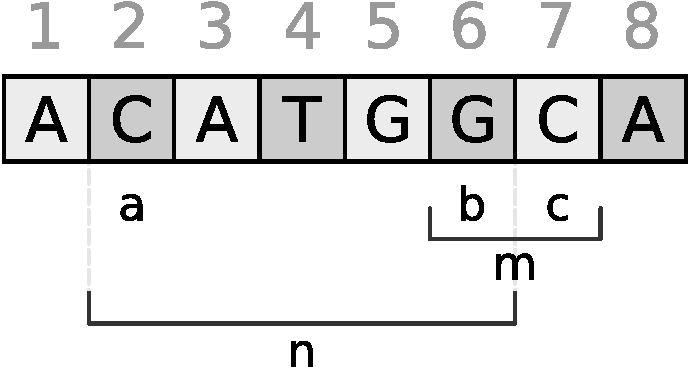
\includegraphics[height=4cm]{figures/sequence.pdf}
    \caption{\small Figure for demonstrating variant types.}
    \label{fig:sequence}
  \end{center}
\end{figure}

\subsection{Example usage}

\begin{siderules}
\begin{verbatim}
vcf2turtle --input-file=/path/to/my/variants.vcf > /path/to/my/variants.ttl
\end{verbatim}
\end{siderules}

\subsection{Run-time properties}

  The program typically uses less than eight megabytes of memory, because it
  processes the variant calls one-by-one.  It reads through the file from top
  to bottom, so its running time is dependent on the input file size.  The
  throughput of this program is around $20$ to $60$ megabytes per second,
  depending on your computer.

\section{Importing data with \texttt{curl}}
\label{sec:curl}

  To load RDF data into a triple store (our database), we can use \texttt{curl}.

  The triple stores typically store data in \emph{graphs}.  One triple store
  can host multiple graphs, so we must tell the triple store which graph we
  would like to add the data to.

\subsection{Example usage}

\begin{siderules}
\begin{verbatim}
curl -X POST                                                 \
     -H Content-Type:text/turtle                             \
     -T /path/to/variants.ttl                                \
     -G <endpoint URL>                                       \
     --digest -u <username>:<password>                       \
     --data-urlencode graph=http://example/graph
\end{verbatim}
\end{siderules}

\chapter{Web interface}
\label{chap:web-interface}

  In addition to the command-line programs, the project provides a web
  interface for prototyping queries, and quick data reporting.  With the
  web interface you can:
  \begin{itemize}
  \item Write and execute SPARQL queries;
  \item Import and export data;
  \item Visualize triple patterns;
  \item View database statistics.
  \end{itemize}

\section{Running the web interface}

  The web interface can be started using the following command:

\begin{siderules}
\begin{verbatim}
web/run
\end{verbatim}
\end{siderules}

  By default, it will be available on \url{http://localhost:5000}.

\section{Prototyping SPARQL queries}

\section{Accessing non-local graphs}

\chapter{Information retrieval with SPARQL}

  In section \ref{sec:vcf2turtle} {\color{LinkGray}`%
  \nameref{sec:vcf2turtle}'} we discussed how to extract
  triples from common data formats.  In section \ref{sec:curl}
  {\color{LinkGray}`\nameref{sec:curl}'} we discussed how we could insert
  those triples into a SPARQL endpoint.

  In this section, we will start exploring the inserted data by using the
  query language called \emph{SPARQL}.  Understanding SPARQL will be crucial
  for the integration in your own programs or scripts --- something we will
  discuss in chapter \ref{chap:programming}
  {\color{LinkGray}`\nameref{chap:programming}'}.

  The queries in the remainder of this chapter can be readily copy/pasted into
  the query editor of the web interface (see chapter \ref{chap:web-interface}
  {\color{LinkGray}`\nameref{chap:web-interface}'}).

\section{Local querying}

  The promise from ``linked data'' is to make data available in such a way that
  one query can retrieve information from multiple SPARQL endpoints.  We call
  querying over multiple SPARQL endpoints \emph{federated querying}.  But before
  we do that, let's look at simple queries that only look at our own data.

\subsection{Retrieving all structural variants}
\begin{siderules}
\begin{verbatim}
PREFIX : <http://localhost:8890/TestGraph/>

SELECT ?variant
WHERE {
  ?variant a :StructuralVariant .
}
\end{verbatim} 
\end{siderules}

\subsection{Retrieving information about structural variants}
\label{sec:sparqling-svs}

\begin{siderules}
\begin{verbatim}
PREFIX : <http://localhost:8890/TestGraph/>

SELECT ?variant ?chromosome ?position ?filter ?quality
WHERE {
  ?variant a :StructuralVariant .
  ?variant :quality ?quality .
  ?variant :genome_position ?p .
  ?variant :filter ?filter .
  ?p :chromosome ?chromosome .
  ?p :position ?position .
}
\end{verbatim}
\end{siderules}

\subsection{Counting structural variants}

\begin{siderules}
\begin{verbatim}
PREFIX : <http://localhost:8890/TestGraph/>

SELECT COUNT(?variant) as ?numberOfVariants
WHERE {
  ?variant a :Variant .
}
\end{verbatim}
\end{siderules}

\subsection{Filtering structural variants}

\begin{siderules}
\begin{verbatim}
PREFIX : <http://localhost:8890/TestGraph/>

SELECT ?variant ?type ?quality ?chromosome ?position
WHERE {
  ?variant a :StructuralVariant .
  ?variant :quality ?quality .
  ?variant :genome_position ?p .
  ?variant :type ?type .
  ?p :chromosome ?chromosome .
  ?p :position ?position .

  FILTER (?position > 80000)
  FILTER (?position < 90000)
  FILTER (?chromosome = "X")
  FILTER (?type = "DEL")
}
\end{verbatim}
\end{siderules}

\subsection{Sorting}

\begin{siderules}
\begin{verbatim}
PREFIX : <http://localhost:8890/TestGraph/>

SELECT ?variant ?chromosome ?position ?quality ?filter
WHERE {
  ?variant a :SNPVariant .
  ?variant :genome_position ?p .
  ?p :chromosome ?chromosome .
  ?p :position ?position .
  ?variant :quality ?quality .
  ?variant :filter ?filter .
  FILTER (?filter = "PASS")
}
ORDER BY ?chromosome DESC(?quality)
\end{verbatim}
\end{siderules}

\subsection{More advanced filtering}

\begin{siderules}
\begin{verbatim}
PREFIX : <http://localhost:8890/TestGraph/>

SELECT ?variant ?quality ?chromosome ?filter
WHERE {
  ?variant a :StructuralVariant .
  ?variant :quality ?quality .
  ?variant :genome_position ?p .
  ?variant :filter ?filter .
  ?variant :genome_position ?p .
  ?p :chromosome ?chromosome .
  ?p :position ?position .

  FILTER (?quality < 0)
  FILTER (?filter != "PASS" 
          AND ?filter != "MinSomaticScore"
          AND ?filter != "MaxDepth")
}
ORDER BY ?chromosome
LIMIT 250
\end{verbatim}
\end{siderules}

\subsection{Basic arithmetics and combining properties}

\begin{siderules}
\begin{verbatim}
PREFIX : <http://localhost:8890/TestGraph/>

SELECT ?variant ?quality ?chromosome ?filter ?confidenceInterval
WHERE {
  ?variant a :StructuralVariant .
  ?variant :quality ?quality .
  ?variant :filter ?filter .
  ?variant :genome_position ?p .
  ?p :confidence_interval_start ?cistart .
  ?p :confidence_interval_end ?ciend .
  ?p :chromosome ?chromosome .
  ?p :position ?position .

  FILTER (?filter = "PASS")
  FILTER (?chromosome > 3)
  BIND( ABS(?cistart) + ABS(?ciend) AS ?confidenceInterval)
}
ORDER BY ?chromosome
LIMIT 250
\end{verbatim}
\end{siderules}

\subsection{Patterns with optional matches}
\begin{siderules}
\begin{verbatim}
PREFIX : <http://localhost:8890/TestGraph/>

SELECT ?variant ?type ?cistart ?ciend
WHERE {
  ?variant a :StructuralVariant .
  ?variant :quality ?quality .
  ?variant :type ?type .
  ?variant :filter ?filter .
  ?variant :genome_position ?p .
  ?p :chromosome ?chromosome .
  ?p :position ?position .

  OPTIONAL {
    ?p :confidence_interval_start ?cistart .
    ?p :confidence_interval_end ?ciend .
  }
}
\end{verbatim}
\end{siderules}

\section{Federated querying}

  Now that we've seen local queries, there's only one more construct we need to
  know about to combine this with remote SPARQL endpoints: the \texttt{SERVICE}
  construct.
  
\subsection{Get an overview of Biomodels (from ENSEMBL)}
\begin{siderules}
\begin{verbatim}
PREFIX sbmlrdf: <http://identifiers.org/biomodels.vocabulary#>
PREFIX sbmldb: <http://identifiers.org/biomodels.db/>

SELECT ?speciesId ?name {
  SERVICE <http://www.ebi.ac.uk/rdf/services/sparql/> {
    sbmldb:BIOMD0000000001 sbmlrdf:species ?speciesId .
    ?speciesId sbmlrdf:name ?name
  }
}
\end{verbatim}
\end{siderules}

\subsection{Get all genes in a region (from ENSEMBL)}
\begin{siderules}
\begin{verbatim}
PREFIX grch38: <http://rdf.ebi.ac.uk/resource/ensembl/89/homo_sapiens/GRCh38/>
PREFIX faldo: <http://biohackathon.org/resource/faldo#>
PREFIX rdf: <http://www.w3.org/1999/02/22-rdf-syntax-ns#>
PREFIX rdfs: <http://www.w3.org/2000/01/rdf-schema#>

SELECT DISTINCT ?gene ?ensemblGeneId ?geneType 
                ?location ?begin ?beginPosition 
                ?end ?endPosition {
    ?location faldo:reference grch38:10 .
    ?location faldo:begin ?begin .
    ?location faldo:end ?end .
    ?begin faldo:position ?beginPosition .
    ?end faldo:position ?endPosition .
    ?ensemblGeneId a ?type ;
          rdfs:label ?label ;
          dc:description ?desc ;
          dc:identifier ?id ;
          faldo:location ?location .
    ?type rdfs:label ?geneType .
    ?ensemblGeneId rdfs:label ?gene .
}
LIMIT 10
\end{verbatim}
\end{siderules}

%% \begin{siderules}
%% \begin{verbatim}

%% \end{verbatim}
%% \end{siderules}

\section{Schema reference}

  In section \ref{sec:sparqling-svs} {\color{LinkGray}`%
  \nameref{sec:sparqling-svs}'}, we used various triple patterns like:

\begin{siderules}
\begin{verbatim}
?variant :genome_position ?p
\end{verbatim}
\end{siderules}

  Where does the \texttt{:genome\_position} property come from?  And are
  there more properties available that we haven't seen yet?

  The schema that describes what can be described is called an \emph{ontology}.
  The triples that the \texttt{vcf2turtle} program outputs are described in
  the \emph{close-to-home} ontology.  In table \ref{table:close-to-home}, a
  complete description of the \emph{close-to-home} ontology can be found.

  \hypersetup{urlcolor=black}
  \begin{table}[H]
    \begin{tabularx}{\textwidth}{ l l l L }
      \headrow
      \textbf{Subject} & \textbf{Predicate} & \textbf{Object}
      & \textbf{Description}\\
      \evenrow
      :Variant & rdf:type & owl:Class
      & \texttt{:Variant} is used as an identifier for describing a variant .\\
      \oddrow
      :GenomePosition & rdf:type & owl:Class
      & \texttt{:GenomePosition} is used to describe the position when mapped
      to a reference genome.\\
    \end{tabularx}
    \caption{\small The triple patterns described by \texttt{vcf2turtle}.}
    \label{table:close-to-home}
  \end{table}
  \hypersetup{urlcolor=LinkGray}

\chapter{Programming in Python, Perl, R, Scheme, C, and/or C++}
\label{chap:programming}

\section{Using SPARQL with R}
\label{sec:sparql-with-r}

  Before we can start, we need to install the \texttt{SPARQL} package from
  \href{https://cran.r-project.org/web/packages/SPARQL/index.html}{CRAN}.

\begin{siderules}
\begin{verbatim}
install.packages('SPARQL')
\end{verbatim}
\end{siderules}

  Once we're set up, we can query like so:

\begin{siderules}
\begin{verbatim}
# Load the library
library('SPARQL')

# Define the endpoint to query.
endpoint <- "http://localhost:8890/sparql"

# Define the actual query to run.
query <- "PREFIX : <http://localhost:5000/cth/>
PREFIX ref: <http://rdf.ebi.ac.uk/resource/ensembl/90/homo_sapiens/GRCh38/>
PREFIX faldo: <http://biohackathon.org/resource/faldo#>
PREFIX rdf: <http://www.w3.org/1999/02/22-rdf-syntax-ns#>
PREFIX rdfs: <http://www.w3.org/2000/01/rdf-schema#>

SELECT DISTINCT ?variant ?svtype ?geneName ?ensemblGeneId ?location {
    ?variant       rdf:type            :StructuralVariant ;
                   :genome_position    ?p ;
                   :filter             ?filter ;
                   :type               ?svtype .
    ?p             :chromosome         ?chromosome ;
                   :position           ?position .
    ?location      faldo:reference     ref:1 ;
                   faldo:begin         ?begin ;
                   faldo:end           ?end .
    ?begin         faldo:position      ?beginPosition .
    ?end           faldo:position      ?endPosition .
    ?ensemblGeneId rdf:type            ?type ;
                   faldo:location      ?location ;
                   rdfs:label          ?geneName .
    FILTER (?chromosome = \"1\")
    FILTER (?position > (?beginPosition) && ?position < (?endPosition))
}
LIMIT 10";

# Run the query
query_data <- SPARQL (endpoint, query)

# Put the results (a data frame) in a separate variable.
query_results <- query_data$results
\end{verbatim}
\end{siderules}

Additional examples can be found in the \texttt{tools/SVPlot/R} directory.

\chapter{Performance tuning}

  During the development and testing of this project, we found that tuning the
  Virtuoso triple store can improve the query performance significantly.
  Therefore, we address performance enhancements for Virtuoso in this chapter.

\section{Hardware}

  When choosing hardware for running a triple store, we attempt to maximize
  \emph{throughput} of the entire triple store.  This means that the slowest
  component of your hardware will determine the overall performance of the
  triple store.

\subsection{Disk lay-out}

\subsection{CPU utilization}

\subsection{Query performance}

\section{Virtuoso}

\subsection{Indexing schemes}

\subsubsection{Column-wise storage}

\begin{siderules}
\begin{verbatim}
CREATE TABLE DB.DBA.RDF_QUAD (
  G IRI_ID_8,
  S IRI_ID_8,
  P IRI_ID_8,
  O ANY,
  PRIMARY key (P, S, O, G) COLUMN
  );
ALTER INDEX RDF_QUAD ON DB.DBA.RDF_QUAD
  PARTITION (S int (0hexffff00));

CREATE DISTINCT NO PRIMARY KEY REF COLUMN INDEX RDF_QUAD_SP
  ON DB.DBA.RDF_QUAD (S, P)
  PARTITION (S int (0hexffff00));

CREATE COLUMN INDEX RDF_QUAD_POGS
  ON DB.DBA.RDF_QUAD (P, O, S, G)
  PARTITION (O varchar (-1, 0hexffff));

CREATE DISTINCT NO PRIMARY KEY REF COLUMN INDEX RDF_QUAD_GS
  ON DB.DBA.RDF_QUAD (G, S)
  PARTITION (S int (0hexffff00));

CREATE DISTINCT NO PRIMARY KEY REF COLUMN INDEX RDF_QUAD_OP
  ON DB.DBA.RDF_QUAD (O, P)
  PARTITION (O varchar (-1, 0hexffff));

CREATE BITMAP INDEX RDF_QUAD_PGOS ON DB.DBA.RDF_QUAD (G, P, O, S)
PARTITION (O VARCHAR (-1, 0hexffff));
\end{verbatim}
\end{siderules}

\end{document}
